\documentclass[11pt,border=5pt]{standalone}
\usepackage{fontspec}
\setmainfont{cmunrm.otf}[BoldFont=cmunbx.otf,ItalicFont=cmunti.otf,BoldItalicFont=cmunbi.otf]
\usepackage{amsmath}
\usepackage{unicode-math}
\setmathfont{NewCMMath-Regular.otf}
\usepackage{tikz}
\usetikzlibrary{arrows.meta,patterns,angles,quotes}
\begin{document}
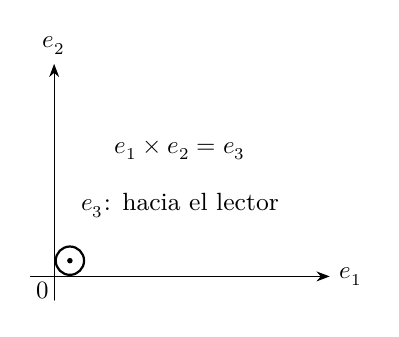
\begin{tikzpicture}[>=Stealth,font=\small,line cap=round,line join=round]
\draw[->,thin] (-0.3,0) -- (3.5,0) node[right] {$e_1$};
\draw[->,thin] (0,-0.3) -- (0,2.7) node[above] {$e_2$};
\node at (-0.14,-0.18) {$0$};
\draw[thick] (.2,.2) circle(.18);\fill(.2,.2) circle(1pt);\node at (1.6,1.6) {$e_1\times e_2=e_3$};
\node at (1.6,0.9) {$e_3$: hacia el lector};

\end{tikzpicture}
\end{document}
